\chapter{Programme und Werkzeuge}

\section{Zeichenkodierung und Umlaute}

Bei Erstellen neuer Dateien bzw. Öffnen und Speichern bereits vorhandener
Dateien ist darauf zu achten, dass stets \gls{utf8} als
\index{Zeichenkodierung}Zeichenkodierung verwendet wird. Dies gilt insbesondere
auch für Quellen des Literaturverzeichnisses (BIB-Dateien).

Umlaute und Zeichen mit \index{Akzent}Akzent werden in den Quelldateien direkt
als solche eingegeben, also direkt \verb#Ä#, \verb#ä#, \verb#ß#, \verb#é#, usw. nicht
\verb#"A#, \verb#"a#, \verb#"ss#, \verb#'e#.

\section{Kommandozeilentools}

Es empfiehlt sich eigentlich die Benutzung einer integrierten
Entwicklungsumgebung, wie z.\,B. TeXnicCenter unter Windows. Diese wird im
folgenden Abschnitt besprochen. Sollte man doch mal in die Verlegenheit kommen
direkt mit den Kommandozeilentools des TeX-Ökosystems arbeiten zu müssen, so
werden nur noch die beiden Tools \texttt{pdflatex} und \texttt{biber} benötigt.
Letzteres erstellt das Literaturverzeichnis. Die Aufrufreihenfolge ist
\begin{verbatim}
#> pdflatex main.tex
#> pdflatex main.tex
#> biber main
#> pdflatex main.tex
#> pdflatex main.tex
\end{verbatim}
Wenn kein \index{Fehler}Fehler aufgetreten ist, sollte nach dem vierten Durchlauf
von \texttt{pdflatex} die \index{Warnung!Please re-run latex}Warnung
\texttt{Please re-run latex} verschwunden sein.

\section{Ubuntu Pakete}
Unter 17.04 sollte es funktionieren, wenn folgende Pakete installiert wurden. Vermutlich reichen auch weniger Pakete:\\
{\small\verb#texlive-bibtex-extra texlive-lang-german texlive-fonts-extra texlive#}\\
{\small\verb#fonts-linuxlibertine biber texmaker#}
(Texmaker ist eine Latex IDE, die aber vermutlich über dependencies schon einige Pakete mitbringt)


\section{IDE Configuration}

Wenn das Build-Kommando von der IDE aus angestoßen werden soll, muss diese entsprechend konfiguiert werden.
TikZ, welches die schönen Graphen malt, möchte gerne Shell Zugriff, dies muss ihm mit dem Paramter {\small\verb#--enable-write18#} (Windows), bzw. {\small\verb#--shell-escape#} (Linux) erlaubt werden.
Außerdem muss statt {\small\verb#"biblatex %.aux"#} für die Referenzen {\small\verb#"biber %"#} genutzt werden.

\section{TeXnicCenter -- Integrierte Entwicklungsumgebung für Windows}

Um nicht obige Kommandos immer per Hand tippen zu müssen, empfiehlt sich die
Verwendung einer integrierten
\index{Entwicklunsumgebung!integrierte}Entwicklungsumgebung; unter \index{Windows}
Windows z.\,B. TeXnicCenter. Für diese Entwicklungsumgebung existiert bereits
eine entsprechende Projektdatei \texttt{thesis.tcp}. Als \texttt{PDF}-Betrachter empfiehlt sich
insbesondere SumatraPDF, da dieser sehr gut mit TeXnicCenter interagiert und
per Doppelklick ein direktes Hin- und Herspringen zwischen Quellcode und
(schadhafter) Stelle im fertigen PDF erlaubt. Unter \index{Linux}Linux eignet
sich die Entwicklungsumgebung Kile.

Da standardmäßig TeXnicCenter von der Verwendung von \gls{bibtex} und nicht
von \gls{biblatex} ausgeht, muss die Konfiguration angepasst werden. Über
den Menüpunkt \texttt{Ausgabe} $\rightarrow$ \texttt{Aus\-ga\-be\-pro\-fi\-le definieren}
den gleichnamigen Dialog aufrufen. Am einfachsten ist es, dass vorhandene Profil
\texttt{LaTeX $\Rightarrow$ PDF} zu kopieren und z.\,B. das Duplikat
\texttt{LaTeX $\Rightarrow$ SumatraPDF + Biber} zu nennen. Die Einstellungen
sind entsprechend \cref{fig:texniccenter-new-profile-1,fig:texniccenter-new-profile-2}
zu ändern.
\begin{figure}[htbp]
\centering
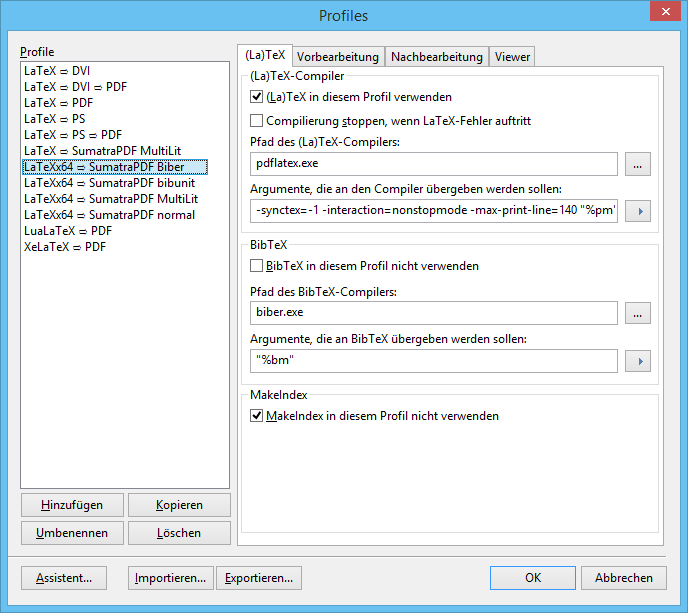
\includegraphics{./images/texniccenter-profile-01.png}
\caption{Neues Ausgabeprofil in TeXnicCenter (1 von 2)}
\label{fig:texniccenter-new-profile-1}
\end{figure}
\begin{figure}[htbp]
\centering
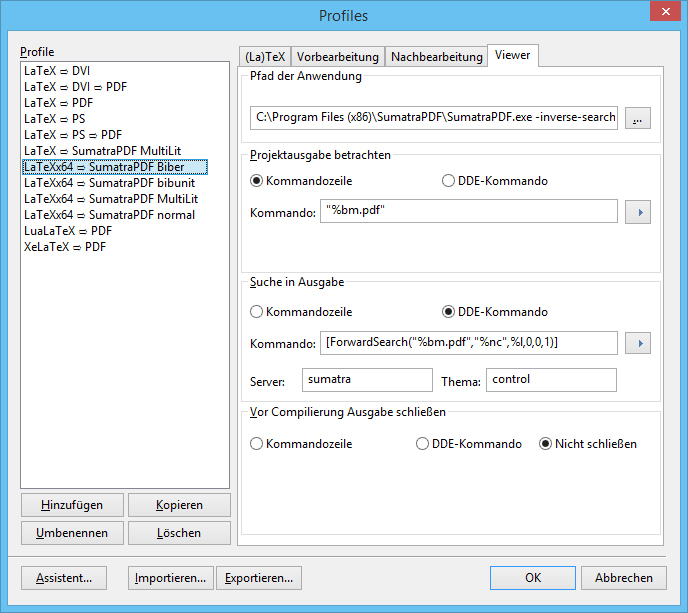
\includegraphics{./images/texniccenter-profile-02.png}
\caption{Neues Ausgabeprofil in TeXnicCenter (2 von 2)}
\label{fig:texniccenter-new-profile-2}
\end{figure}
Im Register \texttt{(La)TeX} ist das \index{Compilerargument}Compilerargument\\
{\small\verb#-synctex=-1 -interaction=nonstopmode -max-print-line=140 "%pm" --enable-write18#}\\
im Register \texttt{Viewer} ist der Anwendungspfad\\
{\small\verb#SumatraPDF.exe -inverse-search "\"TeXnicCenter.exe\" /ddecmd \"[goto('%f','%l')]'\"#}\\

\section{TeXStudio unter Linux}
Zur Konfiguration von TeXStudio muss TexLive manuell installiert werden. Siehe dazu \url{https://wiki.ubuntuusers.de/TeX_Live/#Manuell}. Ansonsten sind die packages nicht kompatibel aufgrund von falschen Versionen. 
Bei der small Installation werden noch einige Packete benötigt, siehe Liste im Git. Dabei muss ausschliesslich \texttt{tlmgr} verwendet werden, um Versionskonflikte zu vermeiden. Um damit installierte Programme zu exportieren und damit aus der Konsole nutzen zu können: \begin{lstlisting}[language=bash]
$ export PATH=/usr/local/texlive/2016/bin/x86_64-linux:$PATH
\end{lstlisting}
Im Git liegt außerdem eine tex-profile \texttt{fraunhofer"=-vorlage"=-thesis"=.txsprofile}. Dann lässt sich mit dem \texttt{Kompilieren} (einfacher grüner Pfeil) Button das Dokument komplett durchkompilieren inklusive Literaturverzeichnis. Zum Bauen ohne Literatur und direktem Anzeigen dient der Button \texttt{Erstellen und Anzeigen} (doppelter grüner Pfeil).
Um das Profil als Standard einzustellen, muss Texstudio als sudo gestartet werden, das Profil unter dem Reiter Optionen geladen werden und anschliessend unter Optionen \texttt{Aktuelle Einstellungen Speichern} gewählt werden. 



\section{TikzEdt}

Hochqualitative Zeichnungen können mit \gls{tikz} erstellt werden. \Gls{tikz} ist jedoch
(analog zu LaTeX) dafür entwickelt worden, den zugehörigen Code per Hand zu
schreiben. Einize \gls{tikz}-Beispiele befinden sich auch in diesem Dokument.
Mit TikzEdt gibt jedoch einen rudimentären \glstext{wysiwyg}-Editor für Windows. Dieser
unterstützt bietet nur eine minimale Unterstützung der \gls{tikz}-Kommandos ist jedoch
hilfreich, um schnell mit optischen Feedback die Kontrollpunkte im
Koordinatensystem festzulegen, bevor dann die weitere Arbeit per Hand erfolgt.


\section{Best Practices MiKTeX}

Unter Windows wird üblicherweise MiKTeX zur Verwaltung von LaTeX-Paketen verwendet. 
Dies funktioniert in den meisten Fällen einwandfrei.
Da die Vorlage jedoch, für LaTeX Verhältnisse, sehr neue und moderne Pakete verwendet, kann es manchmal zu Problemen mit Abhängigkeiten kommen.
Hier sollen Probleme gesammelt werden und auch wie man sie lösen kann.

\subsection{File 'inconsolata.sty' not found}
In der Vorlage wird die Schriftart \emph{inconsolate} verwendet. In MiKTeX 2.9 ist diese Schriftart unter dem Namen \emph{zi4} bekannt.
Es besteht die Hoffnung, dass zukünftig die Schriftart wieder unter dem korrekten Namen verfügbar sein wird.
In der Zwischenzeit hilft es die Datei preamble/01-fonts.tex anzupassen.
\begin{verbatim}
\usepackage[varqu,varl]{inconsolata}
ersetzen durch
\usepackage[varqu,varl]{zi4}
\end{verbatim}

\subsection{Biber und Miktex2.9 x64}
Die Vorlage verwendet BibLaTeX und benötigt dafür das Programm biber.exe.
In der 64 bit Version ist leider aktuell kein Biber enthalten.
Man muss hier\footnote{\url{http://sourceforge.net/projects/biblatex-biber/}}  die für MiKTeX 2.9 die Version 1.9 runterladen und in den Ordner Program Files/MiKTeX 2.9/miktex/bin/x64 kopieren.

\subsection{Windows API error 5: Access is denied}
Wenn man sich entschieden hat, MiKTeX in der Single-User Version zu installieren (was empfohlen wird, um Probleme mit l3kernel zu vermeiden), sind anfänglich die Rechte nicht korrekt gesetzt. 
Deshalb bricht jeder Versuch die MiKTeX Packete zu aktualisieren mit der Fehlermeldung: "`Windows API error 5: Access is denied"' ab.
Um den Fehler zu beheben muss dem eigenen Benutzer Vollzugriff auf den Ordner geben, in dem MiKTeX installiert wurde.

\subsection{package xparse error: support package l3kernel too old}
Dies ist wohl der unerfreulichste Fehler weil die genaue Ursache nicht geklärt ist.
Im Internet finden sich folgende Lösungsideen:
\begin{itemize}
	\item Update von MiKTeX über den Paketmanager
	\item Installation des Pakets "`l3kernel"'
	\item Installation des Pakets "`l3experimental"'
	\item Neuinstallation von MiKTeX
	\item \textbf{Neuinstallation von MiKTeX im Single-User Mode}
\end{itemize}
Bisher konnte das Problem nur durch eine Neuinstallation von MiKTeX im Single-User Mode gelöst werden. Dabei bitte auch den Punkt \textbf{Windows API error 5: Access is denied} beachten.

